\documentclass[a4paper, 12pt]{article}
\usepackage[utf8]{inputenc}
\usepackage[ngerman]{babel}
\usepackage[englisch]{babel}
\usepackage{graphicx}
\usepackage{amsmath}
\usepackage{fixltx2e}
\usepackage{color,soul}
\usepackage{caption}
\usepackage{float}
\usepackage[onehalfspacing]{setspace}
\usepackage{subfig}
\usepackage{geometry}
\usepackage[headsepline]{scrlayer-scrpage}
\usepackage{fancyhdr}
\pagestyle{fancy}
\usepackage{etoolbox}
\usepackage{acronym}
\usepackage{listings}
%\usepackage{minted}

\lstset
{ %Formatting for code in appendix
    language=Matlab,
    basicstyle=\footnotesize,
    numbers=left,
    stepnumber=1,
    showstringspaces=false,
    tabsize=1,
    breaklines=true,
    breakatwhitespace=false,
}
\usepackage{helvet}
\renewcommand{\familydefault}{\sfdefault}

\fancyhead{}
\fancyhead[LO,LE]{Kapitel: \headsection }
%\fancyfoot{}
%\fancyfoot[LE,RO]{Kapitel \thepage}
%\fancyfoot[LO,CE]{\thechapter}

\newgeometry{
   top=2.5cm,
   bottom=2.5cm,
   outer=2.5cm,
   inner=3.5cm,
}

\begin{document}
\thispagestyle{empty} %Verhindert Seitenzahl

\newcommand{\Rule}{\rule{\textwidth}{1mm}}
\begin{center}
    \Rule\vspace{5mm}
    \sffamily\bfseries\Huge
    Untersuchung eines Hybrid-Buck-Wandlers hinsichtlich seiner Anwendbarkeit für Maschine Learning Applikationen
    \vspace{1mm}\Rule
    \vfill  %Einschieben von viel Vertikalem Space
    
\includegraphics[height=16mm]{Pictures/THD-Logo.pdf}
    \vfill
    \LARGE Bachelorarbeit zur Erlangung des akademischen Grades:
   	Bachelor of Engineering
    \vfill
    \Large Sergej Lamert - 00727245 \par
    Fakultät angewandte Informatik \par
    \vfill
    \today
    
\end{center}
\tableofcontents
\newpage
\listoffigures
\section*{Abkürzungsverzeichnis}
\begin{acronym}
\acro{nn}[NN]{Neuronales Netz}
\acro{ml}[ML]{Maschine Learning}
\acro{sda}[SDA]{Serial Data}
\acro{scl}[SCL]{Serial Clock}
\acro{i2c}[I²C]{Inter Integrated Circuit}





\end{acronym}
\section*{Danksagung}

An dieser stelle möchte ich mich bei jedem Bedanken, der mich während dieser Arbeit unterstützt hat. 


Ein großer Dank geht an Andreas Federl, welcher mich sowohl in organisatorischer als auch fachlicher Hinsicht beraten und unterstützt hat.

Ebenfalls bedanken möchte ich mich bei meinen Freunden und meiner Familie, die mich sowohl kreativ als auch mental bei der Arbeit unterstützt haben.
\section*{Abstract}

Die Anwendung von Maschine Learning Algorithmen auf Daten, welche von Hybrid-Buck-Wandler stammen ist momentan nicht weit in der Industrie ausgeprägt. Aus diesem Grund beschäftigt sich diese Arbeit mit der Analyse des o. g. Wandler-Typen hinsichtlich seiner Anwendbarkeit für Maschine Learning Applikationen. Die Analyse beinhaltet die Generierung von Daten, eine Analyse bzgl. der Qualität der Daten sowie der maximalen Abtastrate. Abgeschlossen wird die Analyse mit einem Testfall in Form eines Neuronalen Netzes. Die Ergebnisse der Analyse zeigten, dass die Daten nur geringe Abweichungen von ihrem Mittelwert haben, sowie dass die maximale Abtastrate etwa \hl{Hz} beträgt. Die Anwendung von Neuronalen Netzen anhand von verschiedene periodischen Signalen zeigte eine Genauigkeit von \hl{x}. Zusammenfassend besteht für die in dieser Arbeit behandelten Hybrid-Buck-Wandler Potential für ML Applikationen verwendet zu werden, insofern es sich bei dem Leistungssignal um ein niederfrequentes Signal handelt, da die Daten sonst durch den Alias Effekt unbrauchbar gemacht werden. 
\section{Einleitung}

DC-DC-Buck-Wandler, oder auch Tiefsetzsteller, sind heutzutage Bestandteil verschiedenster Applikationen. So stellen diese beispielsweise Spannung in Notebook-Prozessoren und Ladegeräten zu Verfügung oder regeln den Strom an Stepper-Motoren. Durch die große Anzahl an Anwendungsfällen, ist es besonders in der heutigen Zeit, in der Künstliche Intelligenz und die damit einhergehenden Machine Learning Algorithmen immer wichtiger und präsenter werden, zu evaluieren, inwieweit sich solche Wandler für Machine Learning Anwendungen eignen, wenn Daten über Strom, Spannung, Leistung und Temperatur des Wandlers über eine Digitale Schnittstelle ausgelesen werden können. Deshalb beschäftigt sich diesee Arbeit die Analyse eines Hybrid-Buck-Wandlers für Anwendungen im Bereich des Maschine Learning bzw. der künstlichen Intelligenz.
\\
\\Dadurch bedingt, dass es sich hierbei um einen neu entwickelten Wandler handelt, welcher noch nicht auf dem Markt ist und sich beim Schreiben dieser Arbeit noch in der Testphase befindet, wird die Analyse in mehreren Schritten durchgeführt werden. Zuerst werden in dieser Arbeit allgemeine Testfälle durchgeführt, um die Qualität der Daten sicherzustellen und um einen Einblick in das Verhalten des Wandlers zu gewinnen. Neben der Qualität der Daten muss wird in dieser Arbeit ebenfalls die Quantität der Daten erfasst, dies bedeutet im speziellen, wie viele Daten mit diesem Wandler in einer Zeiteinheit generiert werden können. Des Weiteren wird im Zusammenhang mit dieser Arbeit Software generiert, mit dem die vorhandenen Daten ausgelesen, manipuliert und visualisiert werden können. Schlussendlich ist das Ziel dieser Arbeit, einen ersten Test bezüglich der Anwendbarkeit und Zuverlässigkeit der vom Buck-Wandler generierten Daten für Maschine Learning Applikationen, im speziellen dem der Neuronalen Netze, durchzuführen und zu bewerten.



\section{Theoretischer Hintergrund}
Dadurch bedingt, das diese Arbeit sich an vielen Konzepten aus der Signaltheorie, Elektrotechnik und Informatik bedient, ist es sinnvoll vorab einige Begriffe und Konzepte zu definieren und zu erläutern. Aus diesem Grund, werden im Folgenden das I²C Protokoll, die Grundlagen von Neuronalen Netzen sowie die verwendete Software näher erläutert. 

\subsection{Hybrid-Buck-Wandler}
Bei dem Buck-Wandler handelt es sich um einen DC-DC Wandler, d. h. dieser nimmt eine Gleichstrom Eingangsspannung von 15 bis 40 Volt entgegen und setzt diese herunter auf eine Gleichstrom Ausgangsspannung von 12 Volt. Des Weiteren ist der hier verwendete Wandler auf einen Stromfluss von 10 Ampere limitiert, was bedeutet, dass die maximale Leistung am Ausgang des Wandlers 120 Watt beträgt. Es bedeutet ebenfalls, dass, wenn der Strom 10 A übersteigt, die Ausgangsspannung gedrosselt wird.
Der Wandler besitzt ebenfalls eine I²C Schnittstelle, aus welcher Ausgangsspannung, Eingangsspannung, Ausgangsstrom und Temperatur des Boards gemessen und ausgelesen werden können. Die Datenleitungen des I²C Busses sind bereits auf dem Wandler selbst mit Pull-Up Widerständen ausgestattet, wodurch diese nicht in externen Schaltungen realisiert werden müssen. 

\subsection{I2C}
I2C steht für Inter-Integrated Circuit und wurde von Philips Semiconductors 1982 entwickelt. Es handelt sich dabei um einen seriellen Datenbus im Master-Slave Stil. Dieses Protokoll setzt auf zwei Leitungen für den Datenaustausch, davon ist ein Kanal explizit für die Daten vorgesehen und der andere Kanal für den Takt. Der Takt beträgt im klassischen 100 KHz oder 400 KHz. 


Es ist in Abb. 1 zu erkennen, dass es eine Master- und mehrere Slave Komponenten gibt. Der Master gibt allen Slaves vor, was sie zu senden haben, und wie schnell sie es tun sollen. Des Weiteren ist zu erkennen, das die beiden Leitungen SDA und SCL an einem Pull-Up Widerstand angeschlossen sind. Dieser dient dazu, die Leitungen, wenn weder Master noch Slave sendet, auf die Versorgungsspannung zu schalten, sodass keine undefinierten Zustände entstehen und die Leitung im unbenutzten Zustand eine logische 1 besitzt. Die Kommunikation erfolgt durch Adressen, so besitzt jeder Sensor eine I2C Slave Adresse, über die ein Master auf diese zugreifen kann. Das auslesen der Daten eines Slaves erfolgt per Registeradressen, so hat beispielsweise ein beliebiger I²C fähiger Sensor ein Register, in dem bestimmte Werte gespeichert sind. In dieser Arbeit handelt es sich bei dem I2C Slave um einen Mikrocontroller auf dem Buck-Wandler. Der Master ist dabei ein Raspberry Pi, welcher direkt per I2C mit dem Netzteil verbunden werden kann.
\end{flushleft}


\begin{figure}[H]
    \centering
    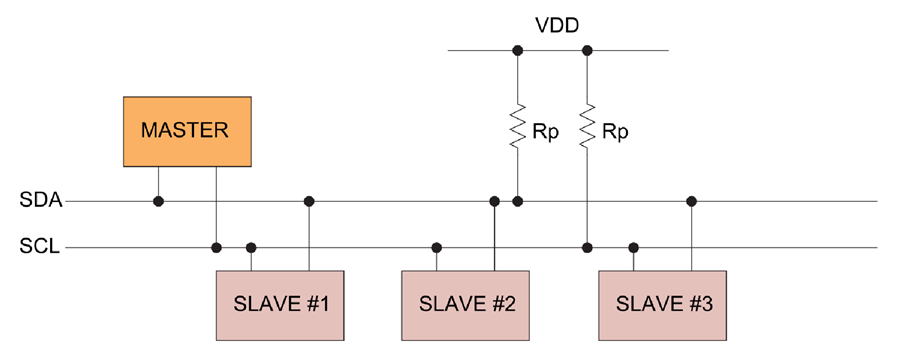
\includegraphics[height= 5cm, width = 10cm]{Pictures/I2C_Bus.png}
    \caption{I2C Bus Beispiel Quelle: https://www.analog.com/en/technical-articles/i2c-primer-what-is-i2c-part-1.html}
\end{figure}

\subsection{Neuronale Netze}

Zur durchführung einiger simpler Testfälle unter den Punkten 3.2.1 und 3.2.2 ist es notwendig, eines der Grundlegenden Konzepte von Machine Learning zu erläutern: das Neuronale Netz.
Neuronale Netze gehören zur Maschine Learning Kategorie des "supervised learning". Beim supervised learning wird ein neuronales Netz anhand von Eingabedaten (Input) und bereits definierten Lösungen (Output) daraufhin optimiert, bei gegebenen Input eine passende Lösungsstrategie für den bereits definierten Output zu finden. 


\begin{figure}[H]
    \centering
    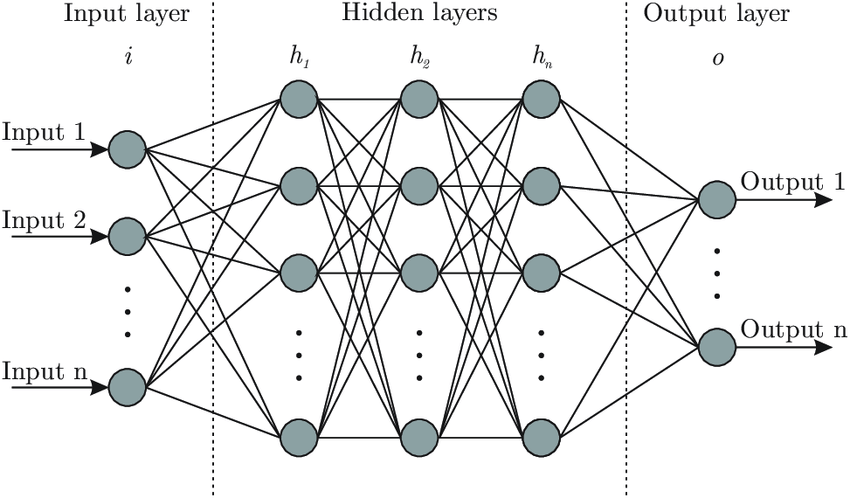
\includegraphics[height= 5cm, width = 10cm]{Pictures/NN_Concept.png}
    \caption{Beispiel eines Neuronalen Netzes: https://www.researchgate.net/figure/Artificial-neural-network-architecture-ANN-i-h-1-h-2-h-n-o_fig1_321259051}
\end{figure}


In Abb. 2 erkennt man eine Abbildung der Architektur eines möglichen neuronalen Netzes. Dieses ist aufgeteilt in mehrere Schichten: Input layer,hidden layer, Output layer. Das Input layer nimmt die Daten auf, welche verarbeitet werden müssen. Diese Daten können von verschiedener Art sein, so können es z. B. Pixeldaten eins Bildes sein, oder der Zeitverlauf von einem Signal. Im hidden layer werden die Daten durch diverse mathematische Operationen verarbeitet, um im Output layer Aussagen über die Input Daten machen zu können, d. h. um die Input Daten zu klassifizieren. Neben den einzelnen Schichten ist zu erkennen, dass es mehrere Knoten gibt, welche untereinander durch Kanten vollvermascht sind. Die Knoten werden im Allgemeinen "Neuronen" genannt und die Kanten sind die sog. "weights\" oder Gewichtungen. Die Gewichtungen sind dabei die Hauptparameter eines Neuronalen Netzes. Bei Neuronalen Netzen wird zwischen zwei Algorithmen unterschieden, dem Feedforward Algorithmus, welcher bei gegebenen Input Daten und Gewichtungen einen bestimmten Output liefert. Und dem Backpropagation Algorithmus, welcher bei gegebenem Input und Output neue Gewichtungen für das Neuronale Netz berechnet. Im Folgenden werden beide Algorithmen näher erläutert. 



\begin{figure}[H]
    \centering
    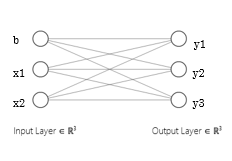
\includegraphics[height= 5cm, width = 6cm]{Pictures/FF.png}
    \caption{Konzept des Feedforward Algorithmus }
    
\end{figure}


    
          A\Bigg(
         \begin{bmatrix}
           w_{10}  w_{11} \\     
           w_{20}  w_{21} \\           
           w_{30} w_{31}
          \end{bmatrix}
          \begin{bmatrix}
           x_{1} \\
           x_{2} \\
         \end{bmatrix}
         + 
         \begin{bmatrix}
           b_{1} \\
           b_{2} \\
           b_{3} \\
         \end{bmatrix}
            \Bigg)
          =
          \begin{bmatrix}
           y_{1} \\
           y_{2} \\
     
           y_{3}
         \end{bmatrix}
         
 	
          }


Abb. 3 zeigt ein vereinfachtes Neuronales Netzt mit zwei Schichten. Das Input layer nimmt zwei Eingangswerte entgegen und verrechnet diese per Matrixmultiplikation mit den Gewichtungen, wie in \hl{Gleichung X dargestellt}. Nach dieser Matrixmultiplikation entsteht ein neuer Vektor mit der gleichen Dimension wie der Output layer. Zu diesem Vektor wird noch der sog. "Bias" addiert. Der Bias dient als feste Skalierung dazu, ein Neuron gezielt mehr, bzw. weniger Aktiv zu machen, das bedeutet mathematisch, dass der numerische Wert gezielt gesteigert bzw. verringert wird. Nachdem der Input mit den Gewichtungen und dem Bias verrechnet wurde, wird auf das Ergebnis eine Aktivierungsfunktion angewendet. Eine Aktivierungsfunktion dient dazu zu bestimmen, wie "aktiv" ein Neuron ist. Es existieren mehrere Aktivierungsfunktionen. So zeigen Abbildungen 4 und 5 zwei Mögliche Funktionen. 

Die Formel für die Sigmoid Funktion: 

\begin{equation}[H]
\label{Sigmoid}
s(z) = \frac{1}{1+e^{-z}}
\end{equation}



In Abb. 4 ist eine der \hl{beliebtesten} Aktivierungsfunktionen zu sehen, die ReLu Funktion. Wenn der Input der Funktion <= 0 ist, dann ist der Output immer 0. Für Werte > 0, ist der Output immer die Identitätsfunktion. Diese Funktion hat den Vorteil, dass sie negative Werte ignoriert, und positive Werte einfach durchlässt. Des Weiteren ist zu erkennen, dass diese Funktion an der Stelle x = 0 nicht differenzierbar ist, da dort ein Knick vorzufinden ist. 


\begin{figure}[H]
    \centering
    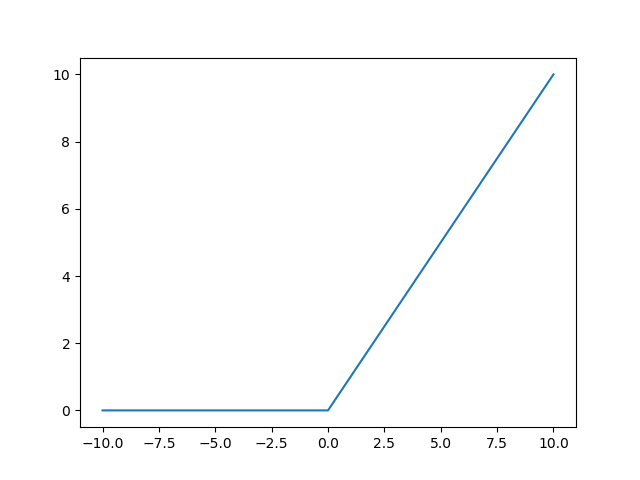
\includegraphics[height= 5cm, width = 10cm]{Pictures/Relu.png}
    \caption{Rectified Linear Unit}
\end{figure}



\[ y = \left\{ \begin{array}{ll}
         0 & \mbox{if $x <= 0$}\\
	        x & \mbox{if $x > 0$}\end{array} \right. \] 
	        
	        
	    


In Abb. 5 ist die Sigmoid Funktion zu erkennen, diese lässt sowohl positive als auch negative Wert durch. Sigmoid ist  im Vergleich zu ReLu jedoch an allen Stellen differenzierbar. 
    
\begin{figure}[H]
    \centering
    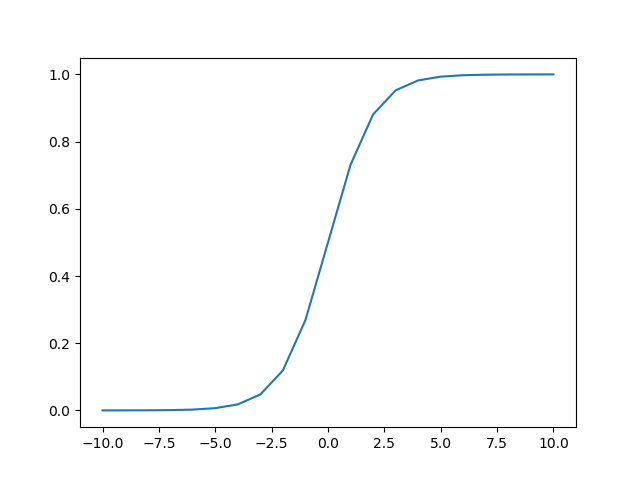
\includegraphics[height= 5cm, width = 10cm]{Pictures/Sigmoid.png}
    \caption{Sigmoid Funktion}
\end{figure}

Der zweite, wichtig Algorithmus für ein Neuronales Netz ist der Backpropagation Algorithmus. Dieser sorgt dafür, dass die vorher erwähnten Gewichtungen an die Input-Output Datenpaare angepasst werden, sodass später korrekte Vorhersagen allein durch die Input Daten gemacht werden können. Für diesen Algorithmus muss eine neue Funktion eingeführt werden: Die Verlustfunktion. Die Verlustfunktion ist eine Funktion in Abhängigkeit der Gewichtungen und sie berechnet den Fehler von den vorhergesagten Daten und den tatsächlichen Daten.

	        
\subsection{Verwendeten Platformen, Programmiersprachen und Bibliotheken}
Zur Datenerhebung per I²C wurde in erster Instanz ein PICkit Serial Analyzer verwendet. Es stellte sich jedoch heraus, dass die Datenrate bei diesem zu gering war, um effektiv Daten zu erheben. Aus diesem Grund wurde für die dynamischen Tests ein Raspberry Pi 4 (4 GB RAM) mit der Programmiersprache Python für Datenerfassung- und Verarbeitung verwendet. Des Weiteren wurde für das Erstellen von Neuronalen Netzen die library "Tensorflow" verwendet, wobei Keras als High-Level API dient. Die graphische Visualisierung der Daten erfolgt ausschließlich per Pyplot library.

\end{flushleft}
\section{Methodik}

\subsection{Datenerfassung}
Dieser Abschnitt beinhaltet verschiedene Ansätze, wie die Daten vom Wandler abgerufen werden können. Dies beinhaltet die Verwendung eines PICkit Serial Analysers sowie die eines Raspberry Pi.


\subsubsection{Notwendigkeit eines Pegelwandlers}
Dadurch bedingt, dass der verwendete Wandler einen Pegel von fünf Volt am I²C Bus besitzt, und ein Raspberry Pi jedoch nur 3.3 Volt, ist es notwendig einen Pegelwandler zwischen die beiden Platinen zu schalten, sodass die Möglichkeit von Hardware defekten ausgeschlossen werden kann. Der dabei verwendete Pegelwandler hat die Bezeichnung TXS0108E. Die Schaltung des Aufbaus ist in Abb. \hl{XX} dargestellt. 

\subsubsection{PICkit Serial Analyzer}
Das Aufzeichnen der Wandler-Daten kann innerhalb zweier Plattformen durchgeführt werden. Eine Plattform ist hierbei ein PICkit Serial Analyzer, der es ermöglicht, auf einem Windows Betriebssystem unter der Verwendung der Programmiersprache C# \hl{Das I²C Protokoll} zu betreiben. Der genannte Serial Analyzer ist in Abb. \hl{X} zu erkennen. Dieser besitzt, wie in der Markierung 6 zu sehen ist mehrere Anschlüsse, welche für verschiedene Protokolle wie I²C, UART und SPI verwendet werden können. Der Quellcode, welcher zur Datenerfassung per PICkit verwendet wurde, ist im \hl{Anhang zu finden}. Der Ablauf des Programms beginnt mit der Definierung verschiedener Funktionen um aus Byte-Daten die tatsächlichen Werte zu berechnen. In der Main Funktion werden zu beginn alle relevante Programmparameter definiert und initialisiert. Dies schließt Adressen, Datenarrays sowie Konfigurationsparameter des PICkit mit ein.  Anschließend erfolgt die Initialisierung des PICkit mit den vorher definierten Parametern. Abgeschlossen wird das Programm durch einen superloop, welche kontinuierlich Daten vom Wandler ausliest, auswertet und in eine Datei abspeichert. \hl{Evtl. noch die Codezeilen mit angeben}

\begin{figure}[H]
    \centering
    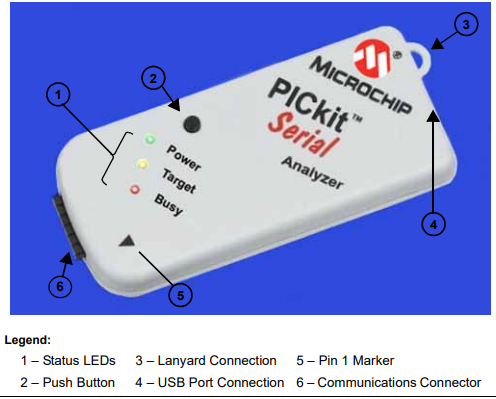
\includegraphics[height= 9cm, width = \textwidth]{Pictures/pickit.png}
    \caption{Strukturierung der gemessenen Daten}
\end{figure}


\subsubsection{Raspberry Pi}
Die zweite Plattform, welche in den Folgenden Tests primär genutzt wird, ist ein Raspberry Pi. Dadurch, dass einem Raspberry Pi sowohl I²C Pins als auch entsprechende Software Libaries zur Verfügung stehen, ist es möglich auch darauf das I²C Protokoll zu nutzen.\\

Es ist ebenfalls wichtig erwähnen, dass die Struktur, in der die Daten innerhalb der Software abgefragt werden relevant ist, da diese sowohl die Abtastrate, als auch die Qualität der Daten beeinflussen kann. So zeigt die Variante 1 des Codes im Anhang eine mögliche Struktur. In dieser werden die einzelnen Parameter separat nacheinander in 2 Byte Blöcken abgefragt. Dies hat den Vorteil, \hl{das die Daten spezifisch abgefragt werden können}. Die Nachteile dieses Verfahrens sind jedoch, ein zusätzlicher Overhead, da durch mehrmaliges Abfragen jedes mal die Adresse des Mikrocontrollers mit angegeben werden muss, was den Datenfluss verlangsamt. Das bedeutet, dass die Adressbits, welche in Abb. \hl{3} dargestellt sind, mit jeder Abfrage mitgeschickt werden müssen. Ein weiterer Nachteil ist, dass die Daten nicht vom selben Zeitabschnitt stammen. So werden beispielsweise, während die Daten aus dem Temperatur Register abgefragt werden, bereits die Daten in den Spannungs- und Stromregistern aktualisiert. \\
\\
Die Abfragestruktur, welche zu bevorzugen ist, ist im Anhang als Variante 2 dargestellt. Diese zeigt, dass alle 8 Bytes des Datenregisters auf einmal ausgelesen werden. Dies hat den Vorteil, dass alle Daten zur gleichen Zeiteinheit abgefragt werden und verhindert zugleich den o. g. Effekt des Overhead, da alle vier Datenregister mit einmaligem versenden der Adresse abgerufen werden. 


\subsection{Speicherung und Strukturierung der Daten}
Die Speicherung der erfassten Daten erfolgt während der Programmlaufzeit. Dieser Umstand bietet sowohl Vor- als auch Nachteile. Ein Nachteil dieser Strategie ist, dass das speichern der Daten nach jeder Abfrage Rechenzeit kostet, was die Abtastrate des Systems verlangsamt. Ein Vorteil dieser Methodik ist jedoch, dass Daten sofort gespeichert werden, und somit nicht die Möglichkeit besteht, dass die Daten bei einem Programmabsturz verloren gehen. Ein weiterer Vorteil besteht darin, dass die Daten nicht im RAM des Raspberry Pi gespeichert werden müssen, da sie mit jeder neuen Datenabfrage auf der Festplatte gespeichert werden, und die Daten im RAM sofort von neuen Daten überschrieben werden. Zusammengefasst kann gesagt werden, dass eine geringe Beeinträchtigung der Abtastrate in kauf genommen wird, für eine geringere Auslastung des RAM und mehr Sicherheit bei der Datenerfassung.

In Abb. \hl{x} ist der Ausschnitt eines Datensatzes zu erkennen. Die Spalten repräsentieren jeweils eine Kategorie von Daten, wie z. B. die Temperatur. Die einzelnen Zeilen beinhalten jeweils einen kompletten Datensatz, welcher in der Zeit aufgenommen wurde, der im Zeitstempel eingetragen ist. Der Zeitstempel hat das Format Stunden:Minuten:Sekunden:Millisekunden.

\begin{figure}[H]
    \centering
    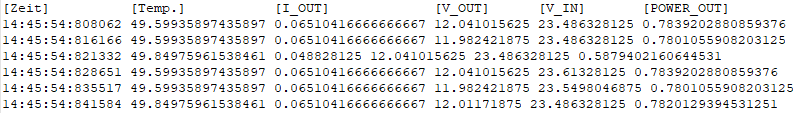
\includegraphics[height= 2.5cm, width = \textwidth]{Pictures/dat_struct.png}
    \caption{Strukturierung der gemessenen Daten}
\end{figure}



\subsection{Methoden der Datenverarbeitung}
In diesem Abschnitt werden die einzelnen Methoden der Datenverarbeitung innerhalb der Software dargestellt. Dies beinhaltet das Laden der Daten, das preprocessing sowie die Visualisierung. Das Laden der Daten erfolgt in der Funktion "unr\_data", welche im Anhang in der Sektion \hl{x} gefunden innerhalb der Zeilen 70 und 117 gefunden werden kann. In dieser Funktion werden die Daten, welche in einer Textdatei gespeichert sind, in eine Matrix gespeichert, welche durch die Library "Numpy" generiert wird. Nachdem die Daten geladen wurden, muss im nächsten Schritt der Zeitverlauf aus den Zeitstempeln generiert werden. \hl{Dies ist deshalb notwendig, da die Daten nicht mit dem Zeitformat "\%H:\%M:\%S:\%f" visualisiert werden können. Aus diesen Zeitstempel werden Zeitdaten in Sekunden generiert.} Sobald die Zeitstempel formatiert wurden, gibt die Funktion in Zeile 117 eine Matrix mit den gemessenen Daten und ein Array mit dem Zeitverlauf aus. Was ebenfalls zu erwähnen ist, ist die For-Schleife am Ende der unr\_data Funktion. Diese Schleife dient dazu Fehler in einem rudimentären Ausmaß zu erkennen. Wie in dem Code zu erkennen ist, werden Datenwerte, welche kleiner als null und größer als Hundert sind als Fehler gehandhabt und können entweder nur zu einem Fehlerzähler hinzu-addiert werden oder direkt dadurch kompensiert werden, indem anstelle des Fehlerhaften Werts der vorher kommende Wert verwendet wird.

Dadurch bedingt, dass alle Signale rauschen, existiert die Möglichkeit einen Software-gesteuerten Tiefpassfilter über das Signal zu legen. Diese Funktion ist zwischen den Zeilen 120 und 125 in der Funktion "apply\_filter" zu erkennen. Diese Funktion kann über die Library "scipy" genutzt werden. 

Eine weitere wichtige Funktion ist "calc\_meta". Diese Funktion dient dazu Metadaten des vorhandenen Datensatzes zu berechnen. Zu den Metadaten gehören: Mittelwert, Länge des Datensatzes, Standardabweichung, numerische Minimum- und Maximum-Werte. Dadurch, dass als Input-Parameter die gesamte Datenmatrix übergeben wird (data), ist die Ausgabe entsprechend eine Matrix in der zu jedem Datensatz (Strom, Spannung, Temperatur) ein Array mit den Metadaten gehört.

Alle bisher genannten Funktionen können genutzt werden, um die Daten abzurufen und zu visualisieren, wie in \hl{den Zeilen} 158 bis 168 aufgezeigt ist. Es werden Daten aus jeder Datei in einem Verzeichnis geladen, Metadaten berechnet sowie ein bestimmtes Signal visualisiert werden.

\subsection{Bestimmung der Abtastrate}
Die Abtastrate des Systems ist durch mehrere Faktoren begrenzt.\hl{Der Verhältnismäßig größte Faktor ist dabei die Taktrate des I²C Busses.} Da diese maßgebend dafür ist, mit was für einem Takt die einzelnen Bits übertragen werden \hl{Siehe Absch. X für i2c}. Der Zweite Faktor, welche die Abtastrate beeinflusst ist die Menge an Daten, die durch das Protokoll übertragen wird. \hl{Dies bedeutet, dass, falls alle Daten des Wandlers abgefragt werden, ergibt dies eine geringere Abtastrate als wenn nur 1 Datenwert abgefragt wird.} Der letzte Aspekt, welcher betrachtet werden muss, ist die Menge an Code, die zwischen den einzelnen Abfragen ausgeführt werden muss. Je mehr Code zwischen nacheinanderfolgenden, periodisch auftretenden, I²C Abfragen liegt, desto langsamer ist die Abtastrate. Aus den o. g. Gründen kann es, je nach Anwendungsfall und Systemeinstellung, zu abweichenden Ergebnissen bei der Abtastrate führen. Deshalb werden die Tests, welche zur Bestimmung der Abtastrate dienen, alle unter gleichen Bedingungen durchgeführt. Dies bedeutet, dass für alle Tests eine I²C Taktrate von 70 KHz eingestellt wird, und der sowohl Code als auch die Datenabfrage nicht verändert werden.



\subsection{Statische Datenerfassung}

Die statische Datenerfassung dient dem Zweck, die Funktionalität der Wandler unter einer konstanten Last zu überprüfen. Es wurden zwei simple Testfälle aufgebaut. Bei beiden handelt es sich um Parallelschaltungen von 4,7 Ohm Widerständen. Der erste Fall schaltet zwei davon parallel, der zweite drei. Durch das Anwenden des Ohmschen Gesetzes, kann ein theoretischer Stromfluss und somit auch die theoretische Leistungsaufnahme berechnet werden. Der Wandler wird durch ein Netzteil mit 24 Volt Ausgangsspannung betrieben. Diese 24 Volt werden von dem Wandler auf 12 V herabgesetzt. Somit kann der Strom berechnet werden, der durch die Widerstände fließt. Bei zwei parallel-geschaltenen Widerständen ergibt das einen theoretischen Stromfluss von 5.1 A wie und bei drei parallel geschaltenen Widerständen 7.65 A wie in den Gleichungen 3 und 4 zu sehen ist.

\begin{equation}
\label{Ohmsches Gesetz}
\frac{U}{R} = I \tab
\end{equation}


\begin{equation}
\label{Ohmsches Gesetz}
\frac{12V}{4.7 \ohm}*2 = 5.10 A 
\end{equation}


\begin{equation}
\label{Ohmsches Gesetz}
12V*4.7 Ohm*3 = 7.65 A 
\end{equation}


Da die statische Datenerfassung über eine konstante Last durchgeführt wird, sind hohe Abtastraten nicht zwingend erforderlich. Aus diesem Grund ist die Nutzung eines PICkit, welcher eine geringe Abtastrate besitzt \hl{nicht problematisch}. Es wird jedoch trotzdem ein Raspberry Pi zur Datenerfassung verwendet, da dieser durch seine höhere Abtastrate eine feinere Ansicht der Daten ermöglicht, wodurch das Rauschen der Daten \hl{besser dargestellt werden kann}. 

\subsection{Dynamische Datenerfassung}

Das Ziel der dynamischen Datenerfassung ist es, zu evaluieren, wie der Wandler sich unter Lasten verhält, die sich mit der Zeit ändern. Sowie mögliche Abweichungen zwischen den einzelnen Wandlern selbst. Der Testaufbau beinhaltet den Hybridwandler, einen Stereoverstärker, welcher per Wandler mit Strom versorgt wird und in den ein Audiosignal eingespeist wird. In Abb. 5 ist die Schaltung des Testaufbaus abgebildet. Es ist zu erkennen, das am Eingang des Buck-Wandlers 24 V eingespeist werden und das die am Ausgang liegenden 12 V an den Stereoverstärker angeschlossen sind. Des Weiteren ist ersichtlich, dass nur ein Kanal des Stereoverstärkers genutzt wird. Dieser Kanal wird mit einem Audiosignal aus einem externen Rechner versorgt. Als Signale werden hierbei Sinussignale mit variierender Frequenz verwendet, welche mit dem Programm Audacity generiert werden. Das Ausgangssignal fällt über einen Lastwiderstand ab. Obwohl es ein Stereoverstärker ist, wurde auf einen Lautsprecher verzichtet, da durch einen Lastwiderstand die Reproduzierbarkeit gewährleistet wird. 


\begin{figure}[H]
    \centering
    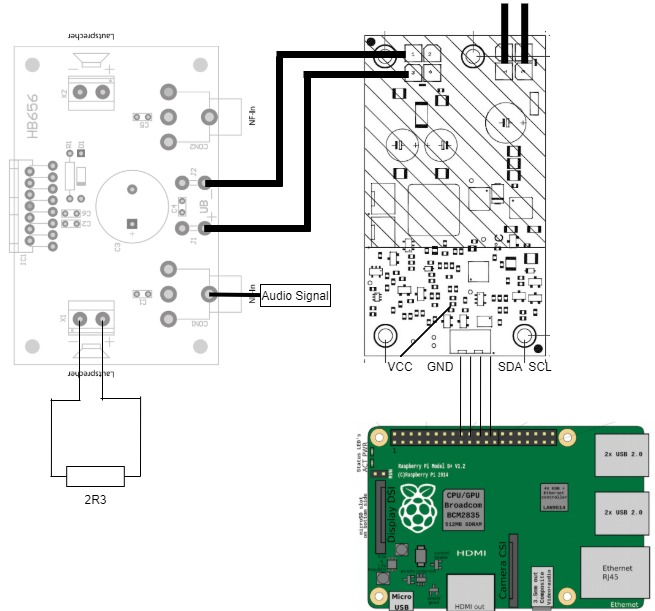
\includegraphics[height= 8cm, width = \textwidth]{Pictures/Dyn_Schaltung.jpg}
    \caption{Versuchsaufbau der dynamischen Datenerfassung}
\end{figure}

Der erste Testschritt ist dabei die Überprüfung, wie hoch die maximale Frequenz eines Signals sein kann, sodass interpretierbare Daten erzeugt werden können. Die maximale Frequenz kann durch praktische Tests empirisch bestimmt werden. Der Umfang dieser Tests besteht darin, die Daten von mehreren Wandlern über einen Zeitraum T zu messen und anschließend die Anzahl der gemessenen Samples durch die gemessene Zeit zu teilen, um so die durchschnittliche Sample-Rate pro Sekunde zu erhalten. 

Dadurch, dass die Datenerfassung auf einem Raspberry Pi abläuft, ist es möglich, die Daten nach jeder Abfrage sofort in eine Textdatei abzuspeichern. Es werden Daten zur Zeit, Temperatur, Ausgangsstrom, Ausgangsspannung und Eingangsspannung aufgezeichnet und tabellarisch abgespeichert.

Die Nyquist-Frequenz stammt aus der Signaltheorie und setzt die maximale Abtastrate in Verhältnis mit der maximalen Frequenz, die ohne Verzerrungen dargestellt werden kann. Die Gleichung besagt, dass die maximale Frequenz, die ohne Verzerrungen dargestellt werden soll, mit einer Abtastrate abgetastet werden soll, die mindestens doppelt so hoch ist, wie die abgetastete Frequenz. Sobald die Abtastrate experimentell bestimmt werden kann, kann das Nyquist-Frequenz theorem darauf angewendet werden, um so die Frequenz zu bestimmen, die maximal mit dem Wandler abgetastet werden kann. 


\subsubsection{Echtzeitmonitoring}
Das Ziel des Echtzeitmonitoring ist es, in laufenden Betrieb des Wandlers Daten zu Strom, Spannung und Temperatur zu erheben, diese Daten zur Verarbeiten und Aussagen darüber zu treffen, welche Last gerade an dem Wandler angeschlossen ist. Eine Last ist in diesem Fall ein Audiosignal, welches durch einen Stereo Verstärker, welcher an den Wandler angeschlossen ist, verstärkt wird. 
Zur Klassifizierung, welche Last, bzw. welches Signal gerade am Stereoverstärker angeschlossen ist, wird ein neuronales Netz verwendet, welches per Tensorflow API generiert wird. Die gemessenen Signale werden dann vom Raspberry Pi, zwecks Verminderung der Rechenleistung, per Socket an einen Rechner geschickt, welcher dann die Daten per Neuronales Netz interpretiert und eine entsprechende Klassifizierung berechnet. Als Testfälle wurden Sinussignal mit verschiedenen Frequenzen verwendet, um die allgemeine Anwendbarkeit von Deep-Learning Algorithmen zu verifizieren. 

\subsubsection{Vergleichsmonitoring mehrerer Wandler im laufenden Betrieb}
Das Ziel des Vergleichsmonitoring ist es, eine Software Struktur aufzubauen, welche es ermöglicht, mehrere Wandler gleichzeitig auf einem Raspberry Pi per I²C zu betreiben und die Daten in Echtzeit zu visualisieren und in Textdateien abzuspeichern. 
 
\hl{wie in Abb. X} zu sehen ist, werden für diesen Testaufbau zwei unterschiedliche Wandler parallel zu einem Netzteil geschaltet, welches 24 V Versorgungsspannung liefert. Die jeweiligen Ausgänge der Wandler werden dann an einen Lastwiderstand angeschlossen. Des Weiteren werden die Ground, SDA und SCL Verbindungen beider Wandler verbunden.

Dadurch, dass die verwendeten Wandler unterschiedlich Adressen besitzen, müssen keine Ergänzungen an der Schaltung durchgeführt werden, es reicht einzig die Datenleitungen (SDA, SCL) zusammenzuschalten. Während der Messung der Wandler, werden die Daten von jedem Messpunkt in Echtzeit auf ein Koordinatensystem per PyPlot übertragen.

\subsection{Anwendbarkeitstest - Neuronales Netz}

Das Ziel des Anwenbarkeitstest ist es zu evaluieren, ob und in welchem Ausmaß sich die vom Wandler generierten Daten sich für Anwendungsfälle im Bereich des Maschine Learning, im speziellen dem der Neuronalen Netze, eignen. Hierfür wird ein simpler Testfall generiert, in dem die Daten mehrerer Signale mit verschiedenen Frequenzen als Input-Daten dienen und der Output entsprechend eine Klassifizierung der Signalfrequenz herausgeben soll.

Als Input-Daten wird der zeitliche Verläufe der Leistung eingespeist. \hl{wie in Abb. x zu sehen ist, bedeutet dass, das t0 - t50 Samples für einen Datensatz verwendet werden. Es ist deshalb bedeutsam die Daten so zu strukturieren, da damit Gewährleistet wird, dass das Neuronale Netz die Daten interpretieren kann, da es sich um zeitlich aufeinanderfolgende Datensamples handelt. In einem Negativbeispiel, in dem nur 1 einziges Sample genommen werden würde, hätte ein NN Probleme damit dieses einzige Sample zu Klassifizieren, da es Teil von verschiedenen Signalen sein kann}

Als Netzwerk Architektur wird ein klassisches vollvermaschtes Neuronales Netz mit zwei Hidden Layern verwendet. Die Anzahl der Neuronen in den Hidden layern muss jedoch praktisch bestimmt werden, damit die besten Resultate erzielt werden können.

\hl{Die entsprechenden Codezeilen sind im Anhang zu zwischen den Zeilen 1 und 50 zu finden.} Darin ist zu erkennen, dass die Trainingsdaten zuerst zufällig gemischt werden, um darauffolgend Normalisiert zu werden. Die in dem Code verwendete Normalisierung ist die "min-max-Normalisierung."  Anschließend wird das Model des Neuronalen Netzes initialisiert. Sobald das Model erstellt wurde, wird es per Befehl "model.compile" mit den gegebenen Trainingsdaten trainiert.


 
Für diese Art von Test ist es unabkömmlich das Nyquist-Frequenz Theorem anzuwenden.  Es ist deshalb so wichtig, da die Daten, die in eine Neuronales Netz eingespeist werden genau einer Kategorie zugewiesen können müssen. Das bedeutet, dass Falls ein Signal mit einer zu niedrigen Abtastrate digitalisiert wird, und sich somit Verzerrungen ergeben, ist nicht mehr gewährleistet, dass die Klassifizierung der ursprünglichen Signalfrequenz erreicht werden kann. Aus diesem Grund müssen für den Anwendbarkeitstest nur Signale mit einer Frequenz verwendet werden, welche nicht durch den Alias-Effekt verzerrt werden.


\section{Ergebnisse}


\subsection{Ergebnisse der statischen Tests}
\begin{flushleft}
Im Folgenden werden die Ergebnisse der statischen Tests mit Bezug auf Temperatur- und Leistungsverlauf mehrerer Wandler dargestellt und näher erläutert. Der Versuchsaufbau und die Testumgebung waren bei allen drei Wandlern nahezu identisch. 
In Abb. 10 ist der Temperaturverlauf [in °C] von drei unterschiedlichen Wandlern  über einen Zeitverlauf von 3600 Sekunden aufgetragen. Es ist zu erkennen, dass der Wandler mit der Bezeichnung 'Board\_10' eine wesentlich höhere Einschwingtemperatur besitzt als die anderen zwei. Dies lässt sich darauf zurückführen, dass besagter Wandler \hl{einen Hardware defekt besitzt}. Des Weiteren ist zu erkennen, dass die beiden verbleibenden Wandler trotz identischer Hardware und gleichen Testbedingungen unterschiedliche Temperaturen vorweisen. \hl{Somit kann behauptet werden, das unter gleichen Bedingungen Abweichende Resultate herauskommen können.}
\end{flushleft}

\begin{figure}[H]
    \centering
    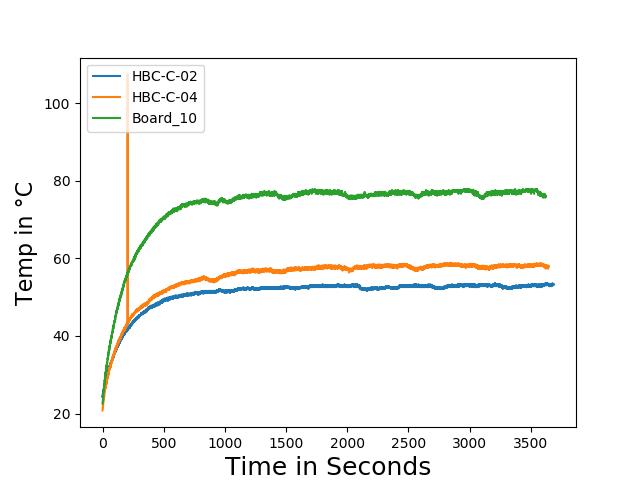
\includegraphics[height= 6cm, width = 12cm]{Pictures/3_Boards_Temp.png}
    \caption{Temperaturvergleich mehrerer Wandler}
\end{figure}


\begin{flushleft}

In \hl{Abb. x} ist der Leistungsverlauf [in Watt] der drei Wandler geplotet gegen die [Zeit in Sekunden] zu sehen. Aus diesem Graphen ist sofort ersichtlich, dass alle Signale rauschen. Wie man \hl{Tabelle X} entnehmen kann, beträgt die Standardabweichung vom Mittelwert bei allen Signalen \hl{Ungefähr 300 Milliwatt}. Die theoretische Leistung, welche bei einer Spannung von 12 V und zwei Parallel geschalteten Widerständen (siehe 3.1) generiert werden müsste, beträgt 61.2 Watt: 

\begin{equation}[H]
\label{Ohmsches Gesetz}
12 V * 5.1 A = 61.2 W 
\end{equation} 

Somit liegt der Wandler mit der Bezeichnung "HB-C-02" am nächsten zum theoretisch berechneten Wert. Diese praktische Abweichung kann durch \hl{einen Leistungsabfall in den Leitungskabeln und der Hardware zumindest teilweise erklärt werden.}

Aufgrund dieser Resultate ist es für Maschine Learning Applikationen sinnvoll auf diese Daten einen Frequenzfilter anzuwenden, um das Rauschen zu eliminieren, da ansonsten Inkonsistenzen bei den K.I Applikationen vorkommen können, da die Daten unter gleichen Bedingungen variieren. 

\end{flushleft}

\begin{figure}[H]
    \centering
    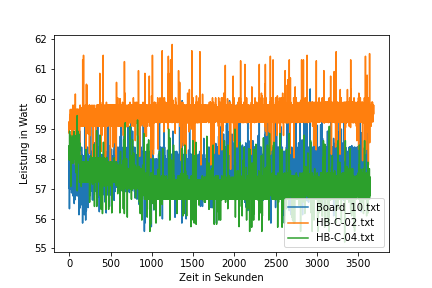
\includegraphics[height= 6cm, width = 12cm]{Pictures/3_Boards_Leistung.png}
    \caption{Leistungsvergleich mehrerer Wandler}
\end{figure}



In \hl{Abb. x} ist der Leistungsverlauf zu erkennen, auf den ein Tiefpassfilter angewendet wurde. Bei dem Tiefpassfilter handelt es sich um \hl{Blablabla details}. Dieser Datensatz besitzt nun kein Rauschen mehr, die einzelnen Signale sind jedoch trotzdem noch unterscheidbar. 


\begin{figure}[H]
    \centering
    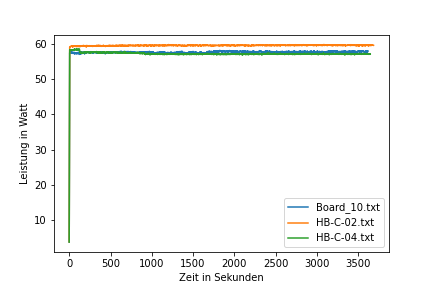
\includegraphics[height= 6cm, width = 12cm]{Pictures/3_Board_Leistung_Filtered.png}
    \caption{Gefilterter Leistungsverlauf der drei Wandler}
\end{figure}

\begin{flushleft}



\subsection{Ergebnisse der dynamischen Tests}
Zur dynamischen Datenerfassung ist zu sagen, dass das I²C Protokoll sich limitierend darauf ausgewirkt hat. Dadurch, dass stabile Programmausführung nur bei einer I²C Taktrate von 70 KHz gewährleistet war, war die Konsequenz daraus, dass die Abtastrate ebenfalls reduziert wurde. Die Ermittlung der Abtastrate erfolgte durch Messungen mehrerer Wandler, die mit verschiedenen Signalen gespeist wurden.Wie in Abb. 13 zu erkennen ist, wurden zwei verschiedene Wandler mit jeweils 6 verschiedenen Signalen verwendet. Zur Bestimmung der jeweiligen Abtastrate wurde zu durch Zeitstempel das Zeitdelta bestimmt, d. h. der Zeitraum in dem die Messungen durchgeführt wurden. Anschließend wurde die Anzahl der aufgenommenen Samples durch das Zeitdelta geteilt, um so auf die durchschnittliche Abtastrate zu kommen. Darauffolgend wurde der Mittelwert von allen Wandler-Signal Paaren berechnet, welcher ~110 Hz beträgt. Wenn auf dieses Ergebnis die oben genannten Konzepte der Nyquist Frequenz angewendet werden, so zeigt sich, dass die maximale Signalfrequenz, welche ohne Verzerrungen durch den Wandler abgetastet werden kann, bei 55 Hz liegt. Aus diesem Grund wurden im nachfolgenden Test mit einem Neuronalen Netz nur Signalfrequenzen verwendet, welche einen geringere Frequenz als 55 Hz besitzen. 

\begin{figure}[H]
    \centering
 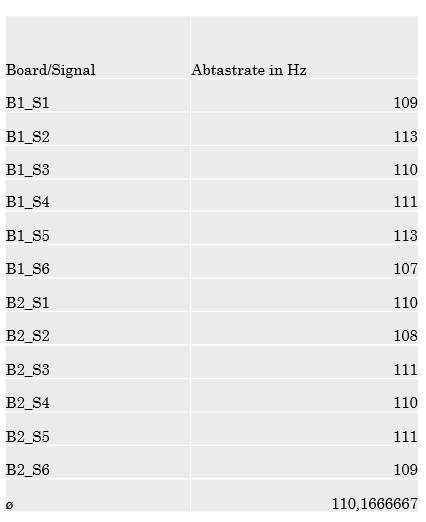
\includegraphics[height= 6cm, width =4 cm]{Pictures/Speed.png}
    \caption{Berechnung der Abtastrate}
\end{figure}


In Abb. 4 ist das generierte Signal zu sehen, welches in den Verstärker eingespeist wird. Dabei handelt es sich in diesem Beispiel um ein 10 Hz Sinussignal, welches in Audacity generiert wurde und als Signalinput für den Stereo-Verstärker dient. Dadurch, dass der Verstärker sowohl positive als auch negative Signale verstärkt, ergibt sich für die reine Leistungsaufnahme des Wandlers eine theoretische Leistungskurve wie sie in Abb. 11 dargestellt ist, nämlich  der Betrag einer Sinusfunktion:

\begin{equation}[H]
f(x) = |sin(2 * pi*x*10)|
\end{equation}

Dadurch, dass es vorher ein Sinussignal mit einer Frequenz von 10 Hz war, ist es nun ein Sinussignal mit einer effektiven Frequenz von 20 Hz.

Das Messen der Daten erfolgte auf einem Raspberry Pi per I²C Protokoll und einer eingestellten Taktrate von 70 KHz, da diese Stabilität gewährleistet. Die Datenerhebung und Verarbeitung erfolgte durch die Programmiersprache Python.

\begin{figure}[H]
    \centering
    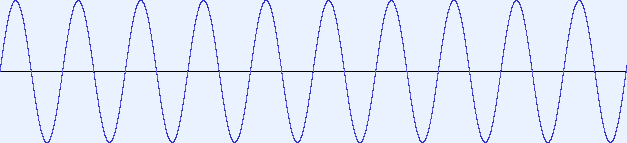
\includegraphics[height= 4cm, width = 12cm]{Pictures/Sinus_Aud.png}
    \caption{In Audacity generiertes 10 Hz Sinussignal}
\end{figure}

\begin{figure}[H]
    \centering
    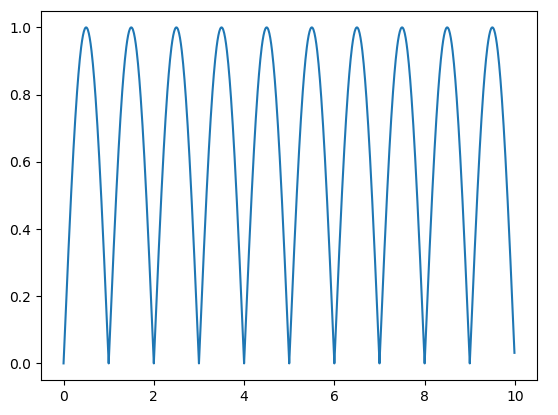
\includegraphics[height= 4cm, width = 12cm]{Pictures/Clapped_Sine.png}
    \caption{Effektive Frequenz eines 10 Hz Signals ist 20 Hz, weil, weil es für den Verstärker egal ist ob + oder - Signal }
\end{figure}

\begin{figure}[H]
    \centering
    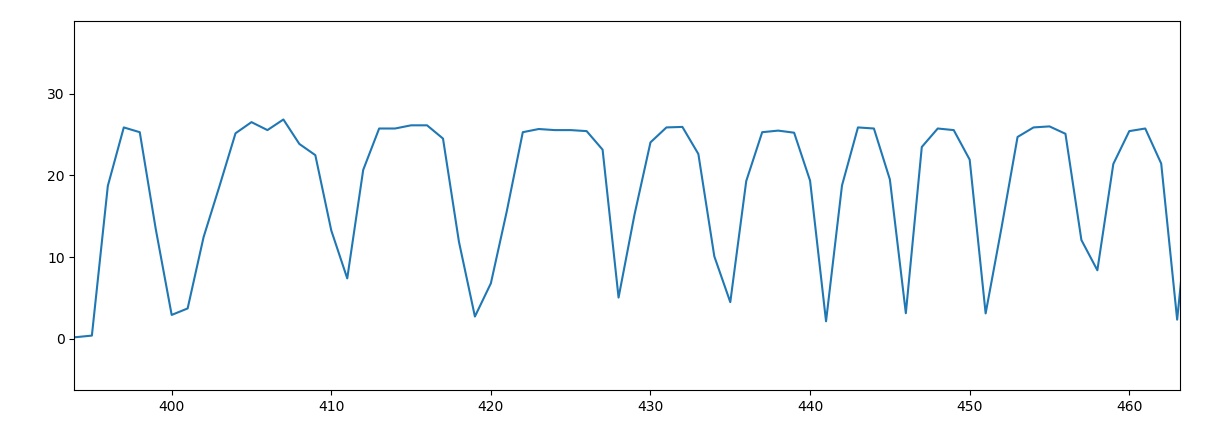
\includegraphics[height= 4cm, width = 12cm]{Pictures/TatsDaten.png}
    \caption{Tatsächlich gemessene Leistung des Wandlers}
\end{figure}


In Abb. 6 ist der ungefilterte Leistungsverlauf des Wandler dargestellt. Es ist ersichtlich, dass das umgeklappte 20 Hz Sinussignal in Abb. 5, dem gemessenen Sinussignal, entspricht. Der unsaubere Verlauf der Leistung ist auf Rauschen innerhalb der Hardware und auf die geringe Abtastrate von 110 Hz zurückzuführen. 


\subsection{Ergebnis des Anwendbarkeitstest - Neuronales Netz}

Als Architektur des Neuronalen Netzes wurde ein Netz mit einem Input layer, zwei Hidden layern, sowie einem Output layer gewählt. Das Input layer hat eine Größe von 50 Neuronen, das bedeutet, dass in einem Datensatz 50 Samples enthalten sind. Die Anzahl der Hidden layer sowie deren Neuronen-Anzahl wurden durch \hl{empirische Tests bestimmt.} Die Anzahl der Output Neuronen entspricht der Anzahl der möglichen Klassifizierungen, in diesem Fall 3 verschiedene Frequenzen: 10 Hz, 20 Hz, 30 Hz. 
Als Aktivierungsfunktion für alle Neuronen, außer die Output Neuronen, wurde ReLu ausgewählt. Der verwendete Optimierungsalgorithmus ist Gradient Descent mit Cross Entropy als Loss-Function.


Abb. 13 zeigt die Genauigkeit des Neuronalen Netzes in der Vorhersage der verschiedenen Frequenzen anhand der Trainingsdaten. Es ist aus dem Graphen ersichtlich, dass die Genauigkeit über 1000 Trainingsepochen ~99\% beträgt. 


\begin{figure}[H]
    \centering
    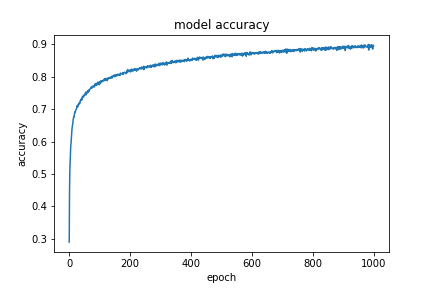
\includegraphics[height= 4cm, width = 8cm]{Pictures/Loss.png}
    \caption{Genauigkeit der Anwendbarkeitstests}
\end{figure}

\section{Fazit und Ausblick}

Die Ergebnisse dieser Arbeit haben gezeigt, das alle verwendeten Wandler in ihrem Leistungssignal rauschen und auch untereinander unter gleichen Bedingungen leicht abweichende Ergebnisse hinsichtlich Strom, Spannung und Leistung liefern.

Des Weiteren konnte gezeigt werden, dass die Wandler eine durchschnittliche stabile Abtastrate von 110 Hz erreichen können, und dass die Daten die dabei generiert werden für Maschine Learning Applikationen verwendet werden können. 
Aus Basis dieser Erkenntnisse können nun weitere, komplexere Tests durchgeführt werden. Diese Tests können auf Signale mit komplexeren Verläufen und höheren Frequenzen angewendet werden.  Ebenfalls können Praxisnähere Tests durchgeführt werden, das bedeutet, dass Hardwarekomponenten verwendet werden und mit dem Wandler mit Strom versorgt werden können, wie z. B. HDD, Raspberry Pi, etc.
\section{Literaturverzeichnis}

https://arxiv.org/abs/1710.05941
Quelle: https://www.analog.com/en/technical-articles/i2c-primer-what-is-i2c-part-1.html
 https://www.researchgate.net/figure/Artificial-neural-network-architecture-ANN-i-h-1-h-2-h-n-o_fig1_321259051
 https://www.fairaudio.de/lexikon/alias-effekt-aliasing/
 https://www.microchip.com/Developmenttools/ProductDetails/DV164122
 https://www.circuitbasics.com/wp-content/uploads/2016/01/Introduction-to-I2C-Message-Frame-and-Bit-2.png
 https://www.ti.com/lit/an/slva704/slva704.pdf?ts=1614862288694&ref_url=https%253A%252F%252Fwww.google.com%252F#:~:text=I2C%20communication%20with%20this%20device,high%20defines%20a%20START%20condition.
 https://www.audacityteam.org/
 https://cdn-reichelt.de/documents/datenblatt/A300/ADAFRUIT_395_ENG_TDS.pdf
\section{Anhang}

Code für PICKIT: 

\begin{lstlisting}{language = [Sharp]C}
using System;
using System.IO;
using System.Text;
using System.Threading;
using System.Threading.Tasks;
using PICkitS;

namespace Bachelor
{
    class Program
    {
        static double Calc_Temp(byte TEMP_HIGH, byte TEMP_LOW)
        {
            int New_High = Convert.ToInt32(TEMP_HIGH);
            int New_Low = Convert.ToInt32(TEMP_LOW);
            int New_High = Convert.ToInt16(TEMP_HIGH);
            int New_Low = Convert.ToInt16(TEMP_LOW);
            New_High = New_High << 8;
            double Temp = New_High + New_Low;
            Temp = ((Temp / 1024 * 5) - 0.4) / 0.0195;
            return Temp;

        }

        static double Calc_I_Out(byte I_Out_High, byte I_Out_Low)
        {
            int New_I_Out_High = Convert.ToInt32(I_Out_High);
            int New_I_Out_Low = Convert.ToInt32(I_Out_Low);
            int New_I_Out_High = Convert.ToInt16(I_Out_High);
            int New_I_Out_Low = Convert.ToInt16(I_Out_Low);

            New_I_Out_High = New_I_Out_High << 8;
            double Amps = New_I_Out_High + New_I_Out_Low;
            Amps = Amps / 1024 * 5 / 0.3;
            return Amps;


        }

        static double Calc_V_Out(byte V_Out_High, byte V_Out_Low)
        {
            int New_V_Out_High = Convert.ToInt32(V_Out_High);
            int New_V_Out_Low = Convert.ToInt32(V_Out_Low);
            int New_V_Out_High = Convert.ToInt16(V_Out_High);
            int New_V_Out_Low = Convert.ToInt16(V_Out_Low);

            New_V_Out_High = New_V_Out_High << 8;
            double Volts = New_V_Out_High + New_V_Out_Low;
            Volts = Volts / 1024 * 5 * 6;
            return Volts;
        }


        static double Calc_V_In(byte V_In_High, byte V_In_Low)
        {
            int New_V_In_High = Convert.ToInt32(V_In_High);
            int New_V_In_Low = Convert.ToInt32(V_In_Low);
            int New_V_In_High = Convert.ToInt16(V_In_High);
            int New_V_In_Low = Convert.ToInt16(V_In_Low);

            New_V_In_High = New_V_In_High << 8;
            double Volts = New_V_In_High + New_V_In_Low;
            Volts = Volts / 1024 * 5 * 13;
            return Volts;
        }




        static void Main(string[] args)
        {
            /*Slave Adress of the Device */
            byte DEV_ADDR_WRITE = 0x10;


            /*Number of Bytes that should be read*/
            byte NUM_BYTES = 0x08;

            /*Registers that I want to read*/
            byte V_IN_ADDR = 0x20;
            byte I_OUT_ADDR = 0x22;
            byte V_OUT_ADDR = 0x24;
            byte TEMP_ADDR = 0x26;

            /*Array where the data gets saved*/
            byte[] Data_Array = new byte[NUM_BYTES];
            Data_Array[0] = 0x20;

            string Script_View = "";

            /*Set Clock speed to 100kHz */
            int Set_Clock = 100;
            double Voltage = 3.3;

            /*Timeout after 2 seconds*/
            int Set_TimeOut = 10000;

            string now = DateTime.Now.ToString("h:mm:ss tt");
            string path = @"C:\Users\lamer\Downloads\Test.txt";
            /*Set Clock speed to 100kHz  and voltage to 3.3 V*/
            int Set_Clock = 400;
            double Voltage = 3.3;

            /*Timeout after 10 seconds*/
            int Set_TimeOut = 100;
       
            string now = DateTime.Now.ToString("h:mm:ss tt");
            string path = @"C:\Users\lamer\Downloads\Board_2_Test_3_Parallel.txt";

            byte High = 0x01;
            byte Low = 0x54;
            double x = Calc_Temp(High, Low);
            Console.WriteLine(x);
            int new_high = Convert.ToInt32(High) << 8;
            int net = new_high + Convert.ToInt32(Low);
            Console.WriteLine(new_high);
            Console.WriteLine(Low);
            Console.WriteLine(net);

            /*Initialisiert den PICKIT, falls mehrere Analyzer verwendet werden, 
            dann die Funktion  Initialize_PICkitSerial mit dem USB Index verwenden 
            Hier ist der USB-Index == 0*/
            if (Device.Initialize_PICkitSerial(0))
            {
                Console.WriteLine("Device Initialization successful");
            }
            else
            {
                Console.WriteLine("Device Initialization failed \n");
                return;
            }
            /*PicKit für I2C Master konfigurieren */
            if (I2CM.Configure_PICkitSerial_For_I2CMaster())
            {
                Console.WriteLine("I2C Master Initialization successful");
            }
            else
            {
                Console.WriteLine("I2C Master Initialization failed \n");
                return;
            }

            if (I2CM.Set_I2C_Bit_Rate(Set_Clock))
            {
                Console.WriteLine("Clock Set successfully to: " + Convert.ToString(Set_Clock));
            }
            else
            {
                Console.WriteLine("Setting Clock failed \n");
                return;
            }

            I2CM.Set_Read_Wait_Time(Set_TimeOut);

            Console.WriteLine("Timeout set to: " + Convert.ToString(Set_TimeOut) + " milliseconds\n");

            //Netzteil hat interne Pull-Ups, daher keine PicKit pullups anmachen        
            if (I2CM.Set_Pullup_State(false))
            {
                Console.WriteLine("Pullups Enabled");
            }
            else
            {
                Console.WriteLine("Pullups could not be enabled");
            }
          
            while (1)
            {
                I2CM.Read(DEV_ADDR_WRITE, V_IN_ADDR, NUM_BYTES, ref Data_Array, ref Script_View);
                double V_IN = Calc_V_In(Data_Array[0], Data_Array[1]);
                double I_OUT = Calc_I_Out(Data_Array[2], Data_Array[3]);
                double V_OUT = Calc_V_Out(Data_Array[4], Data_Array[5]);
                double Temp = Calc_Temp(Data_Array[6], Data_Array[7]);

                now = DateTime.Now.ToString("h:mm:ss");

                string Temp1 = Temp.ToString("0.00");
                string V_OUT1 = V_OUT.ToString("0.00");
                string V_IN1 = V_IN.ToString("0.00");
                string I_OUT1 = I_OUT.ToString("0.00");

                using (StreamWriter w = File.AppendText(path))
                {
                    w.WriteLine(now + " " + Temp1 + " " + V_OUT1 + " " + V_IN1 + " " + I_OUT1);
                }






            }
        }
    }

\end{lstlisting}

\newpage

1. Variante der Datenabfrage: \\

\begin{lstlisting}[language = Python]
def rec_data(device_adress, data_to_send, dcount):
  temp = bus.read_i2c_block_data(device_adress, TEMP_ADDR,2)
  i_out = bus.read_i2c_block_data(device_adress, I_OUT_ADDR,2)
  v_out = bus.read_i2c_block_data(device_adress, V_OUT_ADDR,2)
  v_in = bus.read_i2c_block_data(device_adress, V_IN_ADDR,2)

  temp_high = temp[0]
  temp_low= temp[1]

  i_high = i_out[0]
  i_low = i_out[1]

  v_out_high = v_out[0]
  v_out_low = v_out[1]

  v_in_high = v_in[0]
  v_in_low = v_in[1]

\end{lstlisting}


2. Variante der Datenabfrage: \\
\begin{lstlisting}[language = Python]
from smbus2 import SMBus
import numpy as np
import time
import matplotlib.pyplot as plt
from soundplayer import SoundPlayer
from datetime import datetime
import sys

DEV_ADDR1 = 0x08
V_IN_ADDR = 0x20
I_OUT_ADDR = 0x22
V_OUT_ADDR = 0x24
TEMP_ADDR = 0x26

V_IN_HIST = []
I_OUT_HIST = []
V_OUT_HIST = []
TEMP_HIST = []
POW_HIST = []
data_to_send = np.empty((50))
dcount = 0


def calc_temp(val_high, val_low):
    val = (val_high << 8) + val_low
    Temp = ((val /1024 * 5) -0.4) / 0.0195
    return Temp

def calc_i_out(val_high, val_low):
    val = (val_high << 8) + val_low
    Amps = (val /1024 * 5) / 0.3
    return Amps

def calc_v_out(val_high, val_low):
    val = (val_high << 8) + val_low
    Volt = (val /1024 * 5) * 6
    return Volt


def calc_v_in(val_high, val_low):
    val = (val_high << 8) + val_low
    Volt = (val /1024 * 5) * 13
    return Volt

def rec_data(device_adress, data_to_send, dcount):

  Data = bus.read_i2c_block_data(device_adress, V_IN_ADDR,8)

  temp_high = Data[6]
  temp_low= Data[7]

  i_high = Data[2]
  i_low = Data[3]

  v_out_high = Data[4]
  v_out_low = Data[5]

  v_in_high = Data[0]
  v_in_low = Data[1]


  new_row = []
  current_time = datetime.now().strftime("%H:%M:%S.%f")
  new_row.append(current_time)
  TEMP = calc_temp(temp_high, temp_low)

  new_row.append(TEMP)

  I_OUT = calc_i_out(i_high, i_low)
  new_row.append(I_OUT)

  V_OUT = calc_v_out(v_out_high, v_out_low)
  new_row.append(V_OUT)

  V_IN = calc_v_in(v_in_high, v_in_low)
  new_row.append(V_IN)

  new_row.append(V_OUT*I_OUT)
 
  return new_row

bus = SMBus(1)
while(1):
  try:
     Data1 = rec_data(DEV_ADDR1)
     with open("Test.txt", 'a') as f:
            f.write(str(Data1) + "\n")
   
  except KeyboardInterrupt:
        bus.close()
        sys.exit()
plt.show()

\end{lstlisting}

\newpage
Code für die Datenverarbeitung  \\

\begin{lstlisting}[language = Python]
import numpy as np
import math
import matplotlib.pyplot as plt
import mpld3
import scipy.signal as scys
import enum
from datetime import datetime
import os

def get_measure_time(t1, t2, sample_cnt):
    fmt = '%H:%M:%S:%f'
    t1 = t1#[:-4]
    t2 = t2#[:-4]
    tstamp1 = datetime.strptime(t1,fmt)
    tstamp2 = datetime.strptime(t2,fmt)

    if tstamp1 > tstamp2:
        td = tstamp1 - tstamp2
    else:
        td = tstamp2 - tstamp1
    td_secs = int(round(td.total_seconds()))
    print(td_secs)
    time = []
    print(sample_cnt/td_secs)
    for i in range(0, sample_cnt):
        x = i * td_secs / sample_cnt
        time.append(x)

    with open("Metadata.txt" ,"a") as f:
            f.write(str(sample_cnt/td_secs) + "\n")
    return time

#Enumeration, hat Atm keine Funktionalität
class labels(enum.Enum):
        Temperatur = 1
        Ausgangsspannung = 2
        Eingangsspannung = 3
        Ausgangsstrom = 4
        Leistung = 5
verz = [" in °Celsius", " in Volt", " in Volt", " in Ampere", " in Watt"]

#Metadaten für alle Parameter (Spannung,Strom,Temp) berechnen und in einem 2D Array speichern
def calc_meta(data):
        daten = np.empty((4, 5))
        for i in range(0,4):
            Mittel = np.mean(data[i])
            StandAbw = np.std(data[i])
            len_data = len(data[:][0])
            minimum = np.min(data[i])
            maximum = np.max(data[i])
            daten[i][0] = Mittel
            daten[i][1] = StandAbw
            daten[i][2] = len_data
            daten[i][3] = minimum
            daten[i][4] = maximum
            print("Mittelwert: ", Mittel,  "Standardabweichung: ", StandAbw,
               "Länge: " , len_data,  "Minimum: ", minimum,  "Maximum: ", maximum)
        return daten

#Metadaten z. B. nur für die Temperatur von einem Board berechnen
def calc_meta_single(data):
    Mittel = np.mean(data)
    StandAbw = np.std(data)
    len_data = len(data)
    minimum = np.min(data)
    maximum = np.max(data)
    return Mittel, StandAbw, len_data, minimum, maximum

#Entpacken der Daten aus der Textfile und aufteilen in Zeitverlauf und Daten
def unr_data(path):
        count_samples = 0
        count_errors = 0
        data = np.genfromtxt(path, dtype ='str')
        Daten = np.empty((5, len(data)))

       # with open("Metadata.txt" ,"a") as f:
         #   f.write(path+" ")
        Time = data[:,0]

        #Kleiner Loop um Fehler beim Format zu beseitigen
        #z. B. 08:14:54.56666 -> 08:14:54:56666
        #der Punkt ist ein Fehler der mir beim Daten generieren passiert ist
        for idx,element in enumerate(Time):
            element = np.char.replace(element, '.', ':')
            Time[idx] = element
        Time = get_measure_time(str(Time[0]), str(Time[len(data) -1]), len(data))

        Temp = data[:,1]
        Temp = Temp.astype(np.float32)

        V_OUT = data[:,2]
        V_OUT = V_OUT.astype(np.float32)

        V_IN = data[:,3]
        V_IN = V_IN.astype(np.float32)

        I_OUT = data[:,4]
        I_OUT = I_OUT.astype(np.float32)

        POW = V_OUT * I_OUT

        count_samples += len(data)

        Daten[0] = Temp
        Daten[1] = V_OUT
        Daten[2] = V_IN
        Daten[3] = I_OUT
        Daten[4] = POW

        for i in range(0, 4):
            for j in range(0, len(data)):
                if(Daten[i][j] < 0 or Daten[i][j] > 100):
                    count_errors+=1
                   # Daten[i][j] = Daten[i][j-1]
        print(count_errors)

        return Daten, Time

#Funktion zum Filtern von hohen Frequenzen
def apply_filter(data):
        n = 15
        b = [1.0 / n] * n
        a = 1
        filtered = scys.lfilter(b,a, data)
        return filtered

#Berechnen der Leistung aus Daten
def Calc_Power(Voltage, Current):
        return Voltage * Current


#War eine spielerei, hat at the moment keine Verwendung
def Conf_Plot(Data = None, Time = None, x = None, y = None, Filter = None, Title = None):
        if(Filter == True):
            Data = apply_filter(Data)

        y = labels[y].value
        fig = plt.figure()
        ax1 = fig.add_subplot(211)
        if(x == None):
            ax1.set_ylabel(labels(y).name + verz[y-1])
            ax1.set_xlabel("Zeit in Sekunden")
            ax1.set_title(Title)
            y_mean = [np.mean(Data[y-1])] * len(Data[y-1])
            ax1.plot(Time[:], Data[y-1])#, label= labels(y).name + verz[y] +  vs  + Zeit in Sekunden)
        else:
            x = labels[x].value
            ax1.set_ylabel(labels(y).name + verz[y-1])
            ax1.set_xlabel(labels(x).name + verz[x-1])
            ax1.set_Title(Title)
            ax1.plot(Data[x-1], Data[y-1])#, label= labels(y).name + verz[y-1] +  vs  + labels(x).name + verz[x-1].name)
        ax1.legend(loc ='best')
        plt.savefig(labels(y).name)
        plt.plot()
        plt.show()
        
directory = 'C:\\Users\\lamer\\Downloads\\Bachelor\\Data\\CSV\\'
for filename in os.listdir(directory):

    Data, Time = unr_data(directory+filename)
    x = calc_meta_single(Data[4])
    print(filename,": ", x[0], x[1])

    plt.plot(Time,Data[0], label = filename)
    plt.xlabel('Zeit in Sekunden')
    plt.ylabel('Temperatur in C')
    plt.legend(loc = 2)
    plt.show()

\end{lstlisting}




\newpage

Code für das Neuronale Netz. 
\begin{lstlisting}[language = Python]
import tensorflow as tf
from tensorflow import keras
from tensorflow.keras import layers
import pydot 
import graphviz
import numpy as np
import math
import matplotlib.pyplot as plt
import mpld3
import scipy.signal as scys
import enum
from datetime import datetime

config = tf.compat.v1.ConfigProto()
config.gpu_options.allow_growth = True
config.log_device_placement = True
sess= tf.compat.v1.Session(config=config)

Training_Data = np.concatenate((_5Hz, _20Hz, _30Hz,  __5Hz, __20Hz, __30Hz,___5Hz, ___20Hz, ___30Hz), axis =0)
np.random.shuffle(Training_Data)
Solution = Training_Data[:, Training_Data.shape[1]-1]
Training_Data = Training_Data[:,:-1]
Input_Parameter = Training_Data.shape[1]
Output_Layer_Size = 3
Hidden_Layer_Size = int(Input_Parameter*(2/3)) + Output_Layer_Size
print(Hidden_Layer_Size)



for i in range(0, Training_Data.shape[1]-2):
    max1 = max(Training_Data[:,i])
    min1 = min(Training_Data[:,i])
    Training_Data[:,i] = ( (Training_Data[:,i] - min1) / (max1-min1))
    

with sess:
    model = tf.keras.Sequential(
        [
            layers.Dense(80, input_dim = Input_Parameter,  activation ="relu", name = "Start"),
            layers.Dense(40, activation = "relu", name = "hidden1"),
            layers.Dense(3, activation ="softmax", name = "Output"),
        ]
     )
    model.compile(optimizer = "adam", loss=tf.keras.losses.SparseCategoricalCrossentropy(from_logits=True),
                      metrics=['accuracy'])
    history = model.fit(Training_Data, Solution, epochs = 300)
   
\end{lstlisting}


\end{document}

